\newpage
  
\begin{tcolorbox}

\chapter{2017 - Čez Rob}
	
	\lettrine{A}{fter} the successful 2016 expedition, there was an abundance of high quality leads at shallow levels along the \passage[branch]{Karstaway} branch and beneath \passage{TTT}; the many question marks we had thus left unchecked became the obvious target of the \emph{ Čez Robb} (literally `On the Edge') 2017 expedition. We also expressed the motivation to rig down to the deepest point reached in 2000.

	Over the course of the winter, the JSPDT carried on the exploration of \passage{Monatip}, focussing on the high level horizontal passage connected to \passage{NCB} (the \passage{Avenue of the Pitches}). During the October super action, one particular promising 60\,m pitch was dropped, only to find a tiny trickle of water disappearing through a crack, in the true \passage{Migovec} fashion.

	The summer expedition targeted three main fronts: one branch reached by a traverse over the \passage{Rokovo Brezno} area which, via several pitches connected back to the \passage{Hall of the Mountain King} and the \passage{Karstaway} series; a branch off the \passage{TTT} route, which led to major collapse chambers and still holds promising leads in the far south west of the cave at -500\,m level; a branch below \passage{Smer0}, extended over many trips to a blank area of the mountain with tremendous depth potential and a wide open pitch series at the furthest end.

	A new surface cave, \passage{Jama Gondolin} was discovered after studying a high magnification of a photograph taken the previous year hiking in the \passage{Tolminka} valley. Many similar looking entrances on the western cliffs of \passage{Migovec} await those explorers who do not suffer from vertigo.

\end{tcolorbox}

	\backgroundsetup{	scale=1,
					color=black,
					opacity=1,
					angle=0,
					contents={%
 							 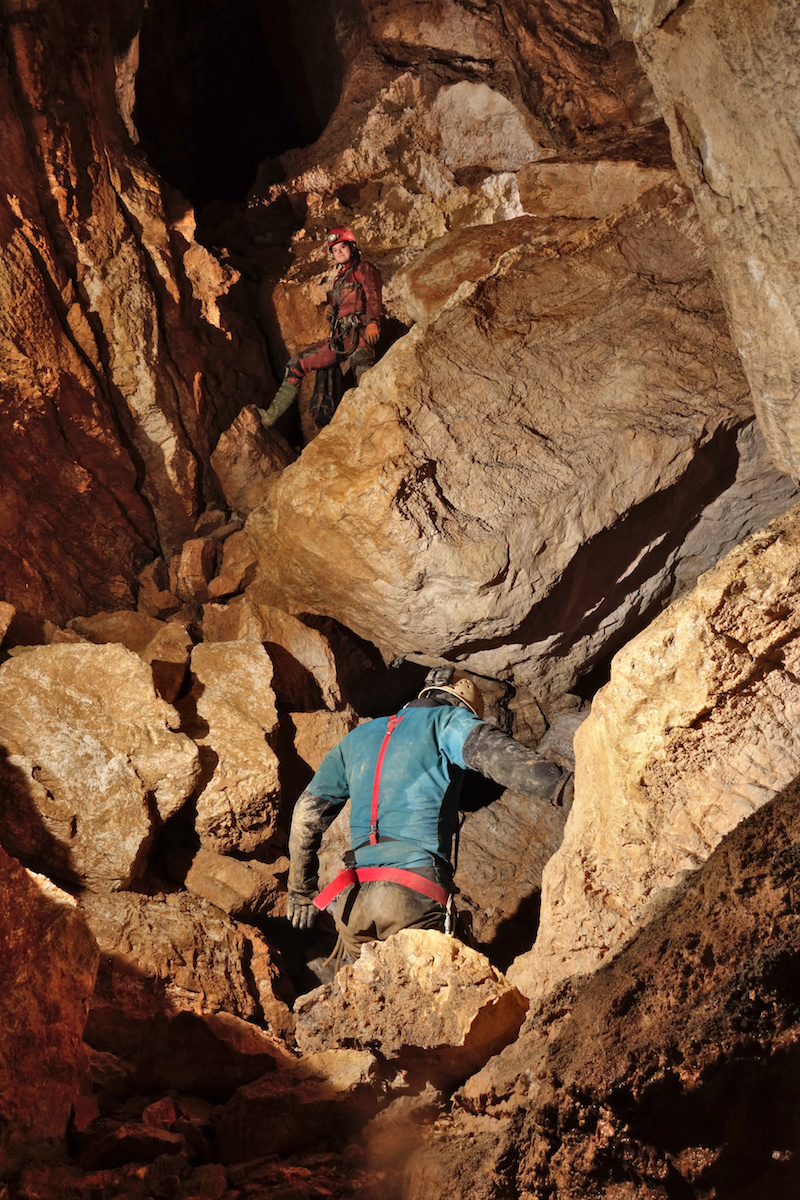
\includegraphics[width=\paperwidth]{images/backgrounds/rhystyers-spiralclimb.jpg}
 					}
	}
\BgThispage
